% =====================================================================
%  07-Compilers-Lexer.tex
%  Technical report of the lexical analyzer - Team 07
%  Compilers, Group 5, Faculty of Engineering, UNAM
%  Compile with pdfLaTeX (Overleaf: Compiler = pdfLaTeX), two passes.
% =====================================================================
\documentclass[11pt,letterpaper]{article}

\usepackage[utf8]{inputenc}
\usepackage[T1]{fontenc}
\usepackage[english]{babel}
\usepackage{lmodern}
\usepackage[margin=2.5cm]{geometry}
\usepackage{amsmath,amssymb}
\usepackage{booktabs,array,tabularx}
\usepackage{xcolor}
\usepackage{listings}
\usepackage{tikz}
\usetikzlibrary{automata,positioning,arrows.meta}
\usepackage{enumitem}
\usepackage{parskip}
\usepackage{caption}
\usepackage{float}
\usepackage{hyperref}

\DeclareUnicodeCharacter{201C}{\textquotedblleft}
\DeclareUnicodeCharacter{201D}{\textquotedblright}

\definecolor{navy}{RGB}{33,54,75}
\definecolor{codebg}{rgb}{0.97,0.97,0.97}
\definecolor{codekw}{rgb}{0.0,0.0,0.6}
\definecolor{codestr}{rgb}{0.6,0.0,0.0}
\definecolor{codecom}{rgb}{0.0,0.45,0.0}

\lstdefinestyle{pycode}{
  language=Python,
  backgroundcolor=\color{codebg},
  basicstyle=\ttfamily\small,
  keywordstyle=\color{codekw}\bfseries,
  stringstyle=\color{codestr},
  commentstyle=\color{codecom}\itshape,
  numbers=left, numberstyle=\tiny\color{gray}, numbersep=6pt,
  breaklines=true, frame=single, showstringspaces=false, tabsize=4,
  literate={á}{{\'a}}1 {é}{{\'e}}1
}
\lstdefinestyle{console}{
  backgroundcolor=\color{codebg},
  basicstyle=\ttfamily\footnotesize,
  breaklines=true, frame=single, showstringspaces=false,
  literate={á}{{\'a}}1
}

\newcommand{\tok}[1]{\texttt{#1}}

\hypersetup{
  colorlinks=true,
  linkcolor=navy,
  citecolor=blue,
  urlcolor=blue,
  linktoc=all,
  bookmarksnumbered=true,
  pdftitle={07-Compilers-Lexer},
  pdfauthor={Team 07 - Compilers, Group 5, FI UNAM}
}

\begin{document}
\sloppy

% =====================================================================
%  COVER PAGE
% =====================================================================
\begin{titlepage}
  \centering
  {\Large\bfseries National Autonomous University of Mexico\par}
  \vspace{0.3cm}
  {\large Faculty of Engineering\par}
  \vspace{2.2cm}
  {\large Compilers\par}
  {\large Group 5\par}
  \vspace{1.8cm}
  {\color{navy}\rule{\linewidth}{1pt}\par}
  \vspace{0.4cm}
  {\Huge\bfseries Lexical Analyzer (Lexer)\par}
  \vspace{0.3cm}
  {\Large Technical Report\par}
  \vspace{0.4cm}
  {\color{navy}\rule{\linewidth}{1pt}\par}
  \vspace{1.8cm}
  {\large\bfseries Team 07\par}
  \vspace{0.6cm}
  \begin{tabular}{ll}
    \toprule
    \textbf{Account number} & \textbf{Role} \\
    \midrule
    321132422 & Presenter \\        % Arzate Rios Adrian Axel
    321237125 & Technical Writer \\ % Bojorquez Covarrubias Evans Martin
    321203018 & Developer \\        % Parra Bello Carlos Enrique
    321135344 & Model Designer \\   % Yanez Barajas Brandon
    321193692 & Project Manager \\  % Zuniga Garcia Hans David
    \bottomrule
  \end{tabular}

  \vfill
  {\large Repository: \url{https://github.com/HansZuniga/Team-07}\par}
  \vspace{0.3cm}
  {\large Package: \texttt{unam.fi.compilers.g5.07}\par}
  \vspace{1cm}
  {\large October 6, 2026\par}
\end{titlepage}

\enlargethispage{3\baselineskip}
\tableofcontents
\newpage

% =====================================================================
\section{Introduction}
% =====================================================================

A compiler translates a program written in a source language into an
equivalent program in another language. This translation is organized in
phases, and the first of them is \textbf{lexical analysis}: the source program
arrives as a plain sequence of characters, and the lexical analyzer
(\emph{lexer} or \emph{scanner}) groups it into meaningful units called
\emph{tokens}, which are then consumed by the syntax analyzer \cite{aho2006}.

This report documents the lexical analyzer developed by Team~07 for the
Compilers course. The program is written in Python~3, does not use the FLEX
tool, and is based on the concepts studied in class: regular expressions,
finite automata and the longest-match policy. It receives a string or a file,
recognizes six token categories (\tok{KEYWORD}, \tok{IDENTIFIER},
\tok{CONSTANT}, \tok{LITERAL}, \tok{OPERATOR} and \tok{PUNCTUATION}), reports
the line and column of each token, reports lexical errors without stopping
the analysis, and displays the total number of tokens found.

The document first presents the problem, the objectives and the theoretical
background; it then describes the formal model built by the team (token
specification, automata, and a context-free grammar with left factoring) and
its implementation; finally, it shows the execution and test results, their
analysis, and the conclusions.

% =====================================================================
\section{Problem Statement and Justification}
% =====================================================================

\subsection{Problem Statement}

The project statement \cite{lexerpdf} asks for a lexical analyzer that:

\begin{itemize}[nosep]
  \item reads an input string or file;
  \item presents basic tokens: at least the keyword \tok{print}, as well
        as identifiers;
  \item displays the sequence of recognized token categories and the
        \textbf{total number of tokens};
  \item processes the reading examples given in the statement
        (\tok{printf("This is an example");} and \tok{int a = 10;}),
        written here with straight quotes (see Section~\ref{sec:limits});
  \item does not use FLEX, either by applying only the theoretical concepts
        seen in class or by using libraries of the programming language;
  \item includes, theoretically, a basic context-free grammar (CFG) that
        represents one of the reading examples, enhanced through
        \emph{left factoring};
  \item is delivered packaged as \tok{unam.fi.compilers.g5.07} in a public
        repository.
\end{itemize}

The core problem is therefore to turn unstructured text into a correctly
classified sequence of tokens, resolving the cases in which the same fragment
could belong to several categories (for example, \tok{int} versus \tok{intx},
or \tok{>} versus \tok{>=}), and handling in a controlled way the characters
that do not belong to the language.

\subsection{Justification}

The lexical analyzer is the foundation of the whole compiler: if tokens are
misclassified, no later phase can work correctly. Moreover, separating
lexical analysis from syntax analysis simplifies the design of the compiler,
improves its efficiency, and isolates the particularities of the input
alphabet \cite{aho2006}.

From an academic point of view, the project makes it possible to apply in a
concrete way the theoretical chain \emph{regular expression $\rightarrow$ NFA
$\rightarrow$ DFA}, as well as the concepts of context-free grammars and left
factoring.

Python was chosen because it allows the team to focus on the
lexical analysis logic and because its \tok{re} module \cite{pythonre}
implements regular expressions in a standard way, so that each pattern in the
program corresponds directly to a regular language in the theoretical model.
A hand-written scanner was preferred over a lexer generator in order to
control precisely the line and column of each lexeme and the error recovery
policy.

% =====================================================================
\section{Objectives}
% =====================================================================

\subsection{General Objective}

To design and implement in Python, without using FLEX, a lexical analyzer that
receives a string or a file, identifies its lexemes, classifies them into
token categories, reports lexical errors, and displays the total number of
valid tokens, supporting its behavior on the theoretical model seen in class.

\subsection{Specific Objectives}

\begin{enumerate}[nosep]
  \item Define the token catalog of the language with its regular
        expressions, examples and priority rules.
  \item Model the representative tokens \tok{IDENTIFIER} and \tok{CONSTANT}
        with an NFA and a DFA, applying $\varepsilon$-closure and the subset
        construction.
  \item Propose a CFG for the example \tok{int a = 10;} and apply left
        factoring to it.
  \item Implement the scanner using the longest-match policy and panic-mode
        error recovery.
  \item Validate the program with an automated test suite that includes the
        professor's examples.
\end{enumerate}

% =====================================================================
\section{Theoretical Background}
% =====================================================================

\subsection{The Lexical Analyzer within the Compiler}

Figure~\ref{fig:phases} shows where the lexical analyzer is located. It reads
the source program character by character, groups the characters into
lexemes, and produces for each one a token that is passed to the syntax
analyzer. Along the way, it discards what is not relevant to the syntax, such
as spaces, tabs and newlines, and keeps track of the position so that errors
can be reported \cite{aho2006}.

\begin{figure}[H]
\centering
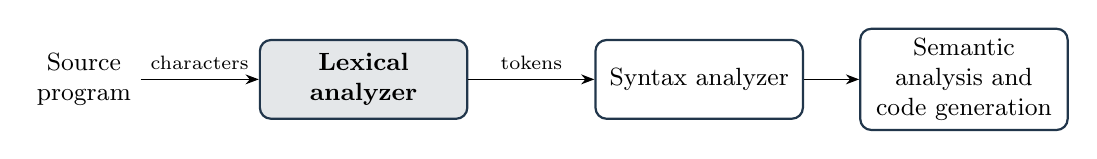
\begin{tikzpicture}[>=Stealth, node distance=0.7cm,
  box/.style={draw=navy, thick, rounded corners, minimum height=1cm,
              text width=2.4cm, align=center, font=\small}]
  \node (src) [font=\small, align=center] {Source\\program};
  \node (lex) [box, right=1.5cm of src, fill=navy!12] {\textbf{Lexical analyzer}};
  \node (par) [box, right=1.6cm of lex] {Syntax analyzer};
  \node (rest) [box, right=of par] {Semantic analysis and code generation};
  \draw[->] (src) -- node[above, font=\scriptsize] {characters} (lex);
  \draw[->] (lex) -- node[above, font=\scriptsize] {tokens} (par);
  \draw[->] (par) -- (rest);
\end{tikzpicture}
\caption{Position of the lexical analyzer among the phases of the compiler.}
\label{fig:phases}
\end{figure}

\subsection{Token, Lexeme and Pattern}

\begin{itemize}[nosep]
  \item \textbf{Lexeme}: a concrete sequence of characters in the source
        program, for example \tok{counter} or \tok{10}.
  \item \textbf{Token}: the category a lexeme belongs to, for example
        \tok{IDENTIFIER} or \tok{CONSTANT}. Formally, it is a pair made of
        the token name and an optional attribute value, such as the lexeme
        itself and its position \cite{aho2006}.
  \item \textbf{Pattern}: a description of the form the lexemes of a token can
        take; in this project, a regular expression.
\end{itemize}

\subsection{Regular Expressions and Finite Automata}

Token patterns describe \textbf{regular languages}, which can be expressed with
regular expressions and recognized by finite automata \cite{hopcroft2007}. A
\textbf{nondeterministic finite automaton (NFA)} may have several transitions
on the same symbol and $\varepsilon$-transitions that consume no input; a
\textbf{deterministic finite automaton (DFA)} has exactly one transition per
symbol from each state. Every NFA can be converted into an equivalent DFA
through:

\begin{itemize}[nosep]
  \item \textbf{$\varepsilon$-closure}, $E(q)$: the set of states reachable
        from $q$ using only $\varepsilon$-transitions.
  \item \textbf{Subset construction}: each DFA state is a set of NFA states;
        from a set $A$ and a symbol $a$ the DFA moves to
        $E(\operatorname{move}(A,a))$. A DFA state is accepting if it contains
        at least one accepting NFA state.
\end{itemize}

\subsection{Longest Match and Priority}

When several patterns could recognize a prefix of the input, lexical
analyzers apply two rules \cite{aho2006}: the \textbf{longest} possible lexeme
is chosen (\emph{maximal munch}) and, if two patterns match the same length,
the one with \textbf{higher priority} wins. Thus, \tok{intx} is one complete
identifier and not \tok{int} followed by \tok{x}, and \tok{>=} is a single
operator.

\subsection{Lexical Errors and Panic Mode}

A lexical error occurs when no pattern matches the prefix of the input. The
simplest recovery strategy is \textbf{panic mode}: the error is recorded,
characters are discarded until scanning can continue, and the analysis goes
on, so that one error does not prevent checking the rest of the program
\cite{aho2006}.

\subsection{Context-Free Grammars and Left Factoring}

A context-free grammar is a tuple $G=(N,T,P,S)$ with nonterminals $N$,
terminals $T$, productions $P$ of the form $A\to\alpha$ with $A\in N$, and a
start symbol $S$. When two alternatives of the same nonterminal share a
prefix, $A\to\alpha\beta_1\mid\alpha\beta_2$, a top-down parser cannot decide
which one to use by looking only at the next token. \textbf{Left factoring}
extracts the common prefix \cite{aho2006}:
\[
A\to\alpha A',\qquad A'\to\beta_1\mid\beta_2 .
\]
The resulting grammar generates the same language, but allows the decision to
be postponed until the common prefix has been read.

% =====================================================================
\section{Development}
% =====================================================================

\subsection{Work Methodology}

The team worked with a Kanban board on GitHub (columns \emph{Backlog},
\emph{Ready}, \emph{In progress}, \emph{Review} and \emph{Done}) and
integrated changes through pull requests. The roles were: Manager (planning,
repository, scope and integration), Model Designer (token specification,
automata and CFG), Developer (implementation), Developer and Model Designer
together (tests), Technical Writer (this report) and Presenter (defense and
demonstration). Design decisions were recorded in \tok{docs/decisions.md} and
the formal model in the \tok{docs/} folder of the repository
\cite{repo}.

\subsection{Token Specification}

Table~\ref{tab:tokens} summarizes the team's token specification as
implemented in the final program. The only difference from the written
specification is in \tok{LITERAL}: the specification also allowed curly
quotes, but the final implementation accepts only straight quotes (see
Section~\ref{sec:limits}). The lexer is case-sensitive, and the identifier alphabet is limited to ASCII letters,
digits and the underscore. Reserved words are read from
\tok{resources/keywords.txt}.

\begin{table}[H]
\centering
\small
\begin{tabularx}{\linewidth}{@{}l>{\raggedright\arraybackslash}p{4.6cm}>{\raggedright\arraybackslash}X@{}}
\toprule
\textbf{Category} & \textbf{Regular expression} & \textbf{Valid / invalid examples} \\
\midrule
\tok{KEYWORD}     & \texttt{print|int|return|if|else} & \tok{int}, \tok{print} / \tok{intx}, \tok{printf} (identifiers) \\
\tok{IDENTIFIER}  & \texttt{[A-Za-z\_][A-Za-z0-9\_]*} & \tok{main}, \tok{\_x}, \tok{if2} / \tok{2a} \\
\tok{CONSTANT}    & \texttt{[0-9]+(?:\textbackslash.[0-9]+)?} & \tok{10}, \tok{0}, \tok{3.14} / \tok{3.}, \tok{123abc}, \tok{1.2.3} \\
\tok{LITERAL}     & \texttt{"[\textasciicircum"\textbackslash r\textbackslash n]*"} & \tok{"Hello"}, \tok{""} / unterminated string \\
\tok{OPERATOR}    & \texttt{==|!=|<=|>=|[=+*/<>-]} & \tok{=}, \tok{>=}, \tok{+} / \tok{\&}, \tok{!} \\
\tok{PUNCTUATION} & \texttt{[()\{\};,]} & \tok{(}, \tok{;}, \tok{\}} / \tok{[}, \tok{]} \\
\bottomrule
\end{tabularx}
\caption{Token catalog and regular expressions.}
\label{tab:tokens}
\end{table}

Priority rules and conflicts:

\begin{itemize}[nosep]
  \item An identifier is read completely before it is reclassified: if the
        lexeme belongs to the set of reserved words it is a \tok{KEYWORD};
        otherwise it is an \tok{IDENTIFIER}. Therefore \tok{if} is a
        \tok{KEYWORD} and \tok{if2} is an \tok{IDENTIFIER}.
  \item Two-character operators (\tok{==}, \tok{!=}, \tok{<=}, \tok{>=}) are
        tried before one-character operators.
  \item Signs are independent operators: \tok{-10} produces an
        \tok{OPERATOR} and a \tok{CONSTANT}.
  \item A string is recognized as a single unit: spaces and operators inside
        it do not produce additional tokens.
  \item Spaces, tabs and newlines are not tokens, but they update the
        position. Lines and columns start at 1.
\end{itemize}

\subsection{NFA/DFA Model}

The two most representative patterns, \tok{IDENTIFIER} and \tok{CONSTANT},
were modeled. In the diagrams, the \emph{start} arrow marks the initial state
and the double circle marks an accepting state. In the tables,
$M=\varnothing$ is the dead state, which absorbs any character.

\subsubsection{Identifiers}

Pattern \texttt{[A-Za-z\_][A-Za-z0-9\_]*}. Let $L$ be an ASCII letter or
underscore and $D$ a digit. The NFA has $Q=\{q_0,q_1,q_2\}$, initial state
$q_0$ and accepting states $F=\{q_2\}$, with
$\delta(q_0,\varepsilon)=\{q_1\}$, $\delta(q_1,L)=\{q_2\}$ and
$\delta(q_2,L)=\delta(q_2,D)=\{q_2\}$ (Figure~\ref{fig:nfa-id}).

\begin{figure}[H]
\centering
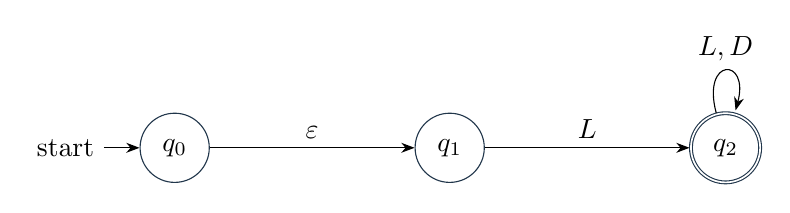
\begin{tikzpicture}[>=Stealth,node distance=2.6cm,every state/.style={draw=navy}]
  \node[state,initial] (q0) {$q_0$};
  \node[state,right=of q0] (q1) {$q_1$};
  \node[state,accepting,right=of q1] (q2) {$q_2$};
  \path[->] (q0) edge node[above] {$\varepsilon$} (q1)
            (q1) edge node[above] {$L$} (q2)
            (q2) edge[loop above] node {$L,D$} (q2);
\end{tikzpicture}
\caption{NFA for \tok{IDENTIFIER}.}
\label{fig:nfa-id}
\end{figure}

The closures are $E(q_0)=\{q_0,q_1\}$, $E(q_1)=\{q_1\}$ and
$E(q_2)=\{q_2\}$. The initial DFA state is $A=E(\{q_0\})=\{q_0,q_1\}$; on
reading $L$, $E(\operatorname{move}(A,L))=\{q_2\}=B$, and from $B$, reading
$L$ or $D$ stays in $B$. $B$ is accepting because it contains $q_2$. The
result is shown in Table~\ref{tab:dfa-id} and Figure~\ref{fig:dfa-id}.

\begin{table}[H]
\centering
\begin{tabular}{lccc}
\toprule
State & $L$ & $D$ & Other \\
\midrule
$\to A=\{q_0,q_1\}$ & $B$ & $M$ & $M$ \\
$*B=\{q_2\}$        & $B$ & $B$ & $M$ \\
$M=\varnothing$     & $M$ & $M$ & $M$ \\
\bottomrule
\end{tabular}
\caption{Transition table of the DFA for \tok{IDENTIFIER}.}
\label{tab:dfa-id}
\end{table}

\begin{figure}[H]
\centering
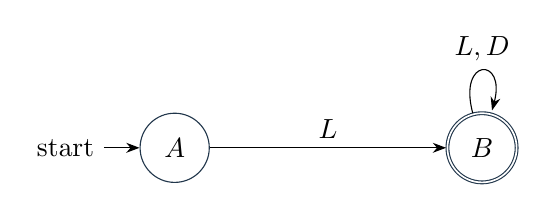
\begin{tikzpicture}[>=Stealth,node distance=3cm,every state/.style={draw=navy}]
  \node[state,initial] (a) {$A$};
  \node[state,accepting,right=of a] (b) {$B$};
  \path[->] (a) edge node[above] {$L$} (b)
            (b) edge[loop above] node {$L,D$} (b);
\end{tikzpicture}
\caption{DFA for \tok{IDENTIFIER} (the dead state $M$ is omitted).}
\label{fig:dfa-id}
\end{figure}

\textbf{Check.} \tok{main}: $A\to B\to B\to B\to B$, accepted; \tok{\_x} and
\tok{if2} are also accepted. \tok{2a}: $A\to M\to M$, rejected. The empty
string stays in $A$, which is not accepting.

\subsubsection{Numeric Constants}

Pattern \texttt{[0-9]+(\textbackslash.[0-9]+)?}. Let $d$ be a digit. The NFA
has $Q=\{q_0,\dots,q_5\}$, initial state $q_0$ and accepting states
$F=\{q_2,q_5\}$ (Figure~\ref{fig:nfa-num}):
\[
\begin{aligned}
\delta(q_0,\varepsilon)&=\{q_1\}, & \delta(q_1,d)&=\{q_2\}, & \delta(q_2,d)&=\{q_2\},\\
\delta(q_2,\varepsilon)&=\{q_3\}, & \delta(q_3,\text{.})&=\{q_4\}, & \delta(q_4,d)&=\{q_5\}, \quad \delta(q_5,d)=\{q_5\}.
\end{aligned}
\]

\begin{figure}[H]
\centering
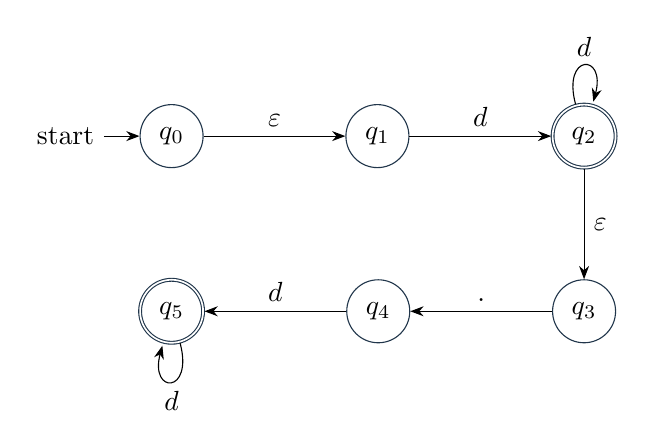
\begin{tikzpicture}[>=Stealth,node distance=1.8cm,every state/.style={draw=navy,minimum size=8mm,inner sep=1pt}]
  \node[state,initial] (q0) {$q_0$};
  \node[state,right=of q0] (q1) {$q_1$};
  \node[state,accepting,right=of q1] (q2) {$q_2$};
  \node[state,below=1.4cm of q2] (q3) {$q_3$};
  \node[state,left=of q3] (q4) {$q_4$};
  \node[state,accepting,left=of q4] (q5) {$q_5$};
  \path[->] (q0) edge node[above] {$\varepsilon$} (q1)
            (q1) edge node[above] {$d$} (q2)
            (q2) edge[loop above] node {$d$} (q2)
            (q2) edge node[right] {$\varepsilon$} (q3)
            (q3) edge node[above] {.} (q4)
            (q4) edge node[above] {$d$} (q5)
            (q5) edge[loop below] node {$d$} (q5);
\end{tikzpicture}
\caption{NFA for \tok{CONSTANT}.}
\label{fig:nfa-num}
\end{figure}

The non-trivial closures are $E(q_0)=\{q_0,q_1\}$ and
$E(q_2)=\{q_2,q_3\}$. By the subset construction: $S=\{q_0,q_1\}$ is the
initial state; $E(\operatorname{move}(S,d))=\{q_2,q_3\}=N$; from $N$, a digit
stays in $N$ and a dot leads to $P=\{q_4\}$; from $P$, a digit leads to
$F_d=\{q_5\}$, which is kept with further digits. $N$ and $F_d$ are accepting
(Table~\ref{tab:dfa-num} and Figure~\ref{fig:dfa-num}).

\begin{table}[H]
\centering
\begin{tabular}{lccc}
\toprule
State & $d$ & Dot & Other \\
\midrule
$\to S=\{q_0,q_1\}$ & $N$   & $M$ & $M$ \\
$*N=\{q_2,q_3\}$    & $N$   & $P$ & $M$ \\
$P=\{q_4\}$         & $F_d$ & $M$ & $M$ \\
$*F_d=\{q_5\}$      & $F_d$ & $M$ & $M$ \\
$M=\varnothing$     & $M$   & $M$ & $M$ \\
\bottomrule
\end{tabular}
\caption{Transition table of the DFA for \tok{CONSTANT}.}
\label{tab:dfa-num}
\end{table}

\begin{figure}[H]
\centering
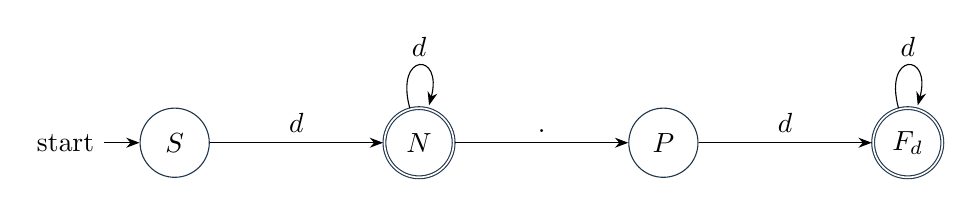
\begin{tikzpicture}[>=Stealth,node distance=2.2cm,every state/.style={draw=navy}]
  \node[state,initial] (s) {$S$};
  \node[state,accepting,right=of s] (n) {$N$};
  \node[state,right=of n] (p) {$P$};
  \node[state,accepting,right=of p] (f) {$F_d$};
  \path[->] (s) edge node[above] {$d$} (n)
            (n) edge[loop above] node {$d$} (n)
            (n) edge node[above] {.} (p)
            (p) edge node[above] {$d$} (f)
            (f) edge[loop above] node {$d$} (f);
\end{tikzpicture}
\caption{DFA for \tok{CONSTANT} (the dead state $M$ is omitted).}
\label{fig:dfa-num}
\end{figure}

\textbf{Check.} \tok{10}: $S\to N\to N$, accepted. \tok{3.14}:
$S\to N\to P\to F_d\to F_d$, accepted. \tok{3.} ends in $P$, which is not
accepting; \tok{123abc} and \tok{1.2.3} reach $M$ and are rejected as
constants.

\subsubsection{Relation to the Program}

The regular expressions \tok{\_IDENTIFIER\_RE} and \tok{\_CONSTANT\_RE} in the
program describe exactly the languages recognized by these DFAs. Python's
\tok{re} module runs each pattern with its own matching engine, so the program
does not build the automata at run time; the model documents the theoretical
equivalence \emph{RegEx $\rightarrow$ NFA $\rightarrow$ DFA} seen in class.
The automata decide whether a complete candidate belongs to the language; the
scanner, in addition, delimits that candidate, applies the longest match, and
reports errors.

\subsection{Context-Free Grammar and Left Factoring}
\label{sec:cfg}

The professor's example \tok{int a = 10;} was chosen, together with the
declaration without initialization \tok{int a;}, so that there are two
alternatives with a common prefix. The grammar works on token categories:
$id$ stands for an identifier and $num$ for a numeric constant, both of them
terminals.

\paragraph{Original grammar.} $G_0=(N_0,T,P_0,S)$ with $N_0=\{S\}$,
$T=\{\texttt{int},id,num,\texttt{=},\texttt{;}\}$ and
\[
S\to\texttt{int}\ id\ \texttt{=}\ num\ \texttt{;}\ \mid\ \texttt{int}\ id\ \texttt{;}
\]
It is context-free because every production has a single nonterminal on its
left-hand side.

\paragraph{Left factoring.} Both alternatives share the prefix
$\texttt{int}\ id$. This prefix is extracted and the nonterminal $R$ is
introduced for the rest:
\[
\begin{aligned}
S &\to \texttt{int}\ id\ R\\
R &\to \texttt{=}\ num\ \texttt{;}\ \mid\ \texttt{;}
\end{aligned}
\]
The new grammar is $G_1=(N_1,T,P_1,S)$ with $N_1=\{S,R\}$. $R\to\texttt{;}$ is
not an empty production: it generates the semicolon of the declaration
without initialization.

\paragraph{Derivations.}
\[
S\Rightarrow\texttt{int}\ id\ R\Rightarrow\texttt{int}\ id\ \texttt{=}\ num\ \texttt{;}
\qquad\qquad
S\Rightarrow\texttt{int}\ id\ R\Rightarrow\texttt{int}\ id\ \texttt{;}
\]

\begin{figure}[H]
\centering
\begin{tikzpicture}[level distance=1.3cm,
  level 1/.style={sibling distance=2.6cm},
  level 2/.style={sibling distance=1.3cm},
  every node/.style={text=navy}]
  \node {$S$}
    child {node {\texttt{int}}}
    child {node {$id$}}
    child {node {$R$}
      child {node {\texttt{=}}}
      child {node {$num$}}
      child {node {\texttt{;}}}};
\end{tikzpicture}
\caption{Parse tree of \tok{int a = 10;} with the factored grammar.}
\label{fig:tree}
\end{figure}

The leaves of the tree (Figure~\ref{fig:tree}), from left to right, are
$\texttt{int},id,\texttt{=},num,\texttt{;}$, which match exactly the token
sequence produced by the lexer for \tok{int a = 10;}:
\tok{KEYWORD IDENTIFIER OPERATOR CONSTANT PUNCTUATION}
(Section~\ref{sec:res}).

\paragraph{Language preservation.}
$L(G_0)=\{\texttt{int}\ id\ \texttt{=}\ num\ \texttt{;},\ \texttt{int}\ id\ \texttt{;}\}$.
In $G_1$, $S$ generates the common prefix and $R$ generates exactly the two
original suffixes, so $L(G_0)=L(G_1)$. The transformation reorganizes the
productions without adding or removing structures, and allows a top-down
parser to choose the production for $R$ by looking at a single token
(\tok{=} or \tok{;}). This grammar covers simple \tok{int} declarations; it is
not intended to be a complete grammar for C, and the lexer does not include a
parser.

\subsection{Implementation}

\subsubsection{Package Architecture}

The repository uses the reverse-domain naming convention, so the requested
package \tok{unam.fi.compilers.g5.07} is located under the folder
\tok{mx/unam/fi/compilers/g5/07}. The package separates code, resources,
examples and tests:

\par\noindent\begin{minipage}{\linewidth}
\begin{lstlisting}[style=console]
mx/unam/fi/compilers/g5/07/
|-- resources/keywords.txt       Reserved words
|-- examples/example_profesor.c  Professor's reading example
|-- src/main/
|   |-- lexer.py                 Token and Lexer classes (core)
|   `-- main.py                  Entry point (command line)
`-- tests/
    |-- conftest.py              pytest configuration
    `-- test_lexer.py            29 automated tests
\end{lstlisting}
\end{minipage}\par\smallskip

Each token is represented by the \tok{Token} class, which stores four fields:
type, lexeme, line and column. The \tok{Lexer} class loads the reserved words,
scans the text, and keeps the valid tokens and the errors in separate lists.

\subsubsection{Compiled Patterns}

The patterns in Table~\ref{tab:tokens} are compiled only once, when the module
is loaded (Listing~\ref{lst:patterns}). The auxiliary pattern
\tok{\_NUMERIC\_CANDIDATE\_RE} is deliberately more permissive than
\tok{\_CONSTANT\_RE}: it captures everything that looks like an attempt at a
number so that it can then be validated as a whole.

\par\noindent\begin{minipage}{\linewidth}
\begin{lstlisting}[style=pycode, caption={Compiled patterns in \tok{lexer.py}.}, label={lst:patterns}]
_NUMERIC_CANDIDATE_RE = re.compile(r"[0-9][0-9A-Za-z_.]*")

_CONSTANT_RE = re.compile(r"[0-9]+(?:\.[0-9]+)?")
_IDENTIFIER_RE = re.compile(r"[A-Za-z_][A-Za-z0-9_]*")
_LITERAL_RE = re.compile(r'"[^"\r\n]*"')
_OPERATOR_RE = re.compile(r"==|!=|<=|>=|[=+*/<>-]")
_PUNCTUATION_RE = re.compile(r"[(){};,]")
\end{lstlisting}
\end{minipage}\par\smallskip

\subsubsection{Scanning Algorithm}

The \tok{tokenize()} method scans the text from left to right with an index
\tok{pos} and line and column counters. At each position it tries the
following cases, in this order:

\begin{enumerate}[nosep]
  \item Newline: advances the line and resets the column to 1.
  \item Space or tab: produces no token; the column advances by 1.
  \item Double quote: tries to read a complete string; if it is not closed on
        the same line, an error is recorded.
  \item Identifier: reads the longest identifier and reclassifies it as a
        \tok{KEYWORD} if it belongs to the set of reserved words.
  \item Numeric candidate: reads it completely and validates it against
        \tok{\_CONSTANT\_RE}; if it does not match as a whole, it is an error.
  \item Operator (two-character operators first), then punctuation.
  \item Any other character: one-character error, and the scanner advances
        one position (panic mode).
\end{enumerate}

Listing~\ref{lst:scan} shows steps 4 and 5, which contain the longest-match
and reclassification rules.

\par\noindent\begin{minipage}{\linewidth}
\begin{lstlisting}[style=pycode, caption={Recognition of identifiers, keywords and constants.}, label={lst:scan}]
# Identifiers and keywords.
match = _IDENTIFIER_RE.match(text, pos)
if match:
    lexeme = match.group()
    token_type = "KEYWORD" if lexeme in self.keywords else "IDENTIFIER"
    self._add_token(token_type, lexeme, line, column)
    pos, column = self._advance(pos, column, len(lexeme))
    continue

# Numeric constants (and malformed numeric candidates).
match = _NUMERIC_CANDIDATE_RE.match(text, pos)
if match:
    candidate = match.group()
    if _CONSTANT_RE.fullmatch(candidate):
        self._add_token("CONSTANT", candidate, line, column)
    else:
        self._add_error(candidate, line, column)
    pos, column = self._advance(pos, column, len(candidate))
    continue
\end{lstlisting}
\end{minipage}\par\smallskip

Because \tok{\_IDENTIFIER\_RE} is greedy, it reads \tok{intx} completely
before checking the set of reserved words, so it is never split into \tok{int}
and \tok{x}. For operators, the order of the alternatives in
\tok{\_OPERATOR\_RE} makes \tok{>=} be tried before \tok{>}.

\subsubsection{Lexical Error Handling}

Three kinds of error are distinguished, all of them reported with their
lexeme and starting line and column:

\begin{enumerate}[nosep]
  \item \textbf{Malformed number}: a candidate that starts with a digit and
        continues with letters, underscores or dots (\tok{123abc}, \tok{3.},
        \tok{1.2.3}) is reported as a single error; it is never split into
        partially valid tokens.
  \item \textbf{Unterminated string}: it is consumed up to the newline or the
        end of the input and reported as a single error.
  \item \textbf{Illegal character}: any other character (\tok{@}, \tok{\&},
        \tok{[}, accented letters) is reported and the scanner advances one
        character.
\end{enumerate}

Errors are stored separately and are \textbf{not added} to the total number
of valid tokens. The analysis always continues with the rest of the input.

\subsubsection{Input and Output}

The program is run from \tok{src/main/} with \tok{main.py}, which accepts a
file or a string; with no arguments, it analyzes the professor's example:

\par\noindent\begin{minipage}{\linewidth}
\begin{lstlisting}[style=console]
python main.py                                     # professor's example
python main.py --file ../../examples/example_profesor.c
python main.py --text "int a = 10;"
\end{lstlisting}
\end{minipage}\par\smallskip

The output is a table with the type, lexeme, line and column of each token;
if there are errors, a second table lists them; and at the end the line
\tok{Total of tokens: N} is printed (plus \tok{Total of lexical errors: M} when
applicable).

% =====================================================================
\section{Results}
\label{sec:res}
% =====================================================================

All the outputs in this section are real executions of the final version of
the repository \cite{repo} (branch \tok{main}, commit \tok{f967b8d}). After
the first example, the table headers (\tok{TYPE LEXEME LINE COLUMN}, the
dashed lines and the header of the error table) are omitted to save space;
the data is unchanged.

\subsection{Professor's Reading Example}

\par\noindent\begin{minipage}{\linewidth}
Input (\tok{examples/example\_profesor.c}):\par\smallskip
\begin{lstlisting}[style=console]
printf("This is an example");
int a = 10;
\end{lstlisting}
\end{minipage}\par\smallskip

\par\noindent\begin{minipage}{\linewidth}
Output of \tok{python main.py}:\par\smallskip
\begin{lstlisting}[style=console]
TYPE         LEXEME                    LINE   COLUMN
----------------------------------------------------
IDENTIFIER   'printf'                  1      1
PUNCTUATION  '('                       1      7
LITERAL      '"This is an example"'    1      8
PUNCTUATION  ')'                       1      28
PUNCTUATION  ';'                       1      29
KEYWORD      'int'                     2      1
IDENTIFIER   'a'                       2      5
OPERATOR     '='                       2      7
CONSTANT     '10'                      2      9
PUNCTUATION  ';'                       2      11

Total of tokens: 10
\end{lstlisting}
\end{minipage}\par\smallskip

The category sequence of the second line is
\tok{keyword identifier operator constant punctuation}, identical to the
expected output shown in the statement (5 tokens). The first line produces 5
more tokens, for a total of 10. \tok{printf} is classified as an identifier
because it does not belong to the set of reserved words.

\subsection{Reserved Words and Two-Character Operators}
\label{sec:reserved}

\par\noindent\begin{minipage}{\linewidth}
\tok{python main.py -{}-text "if (x >= 10) return x; else return 0;"}\par\smallskip
\begin{lstlisting}[style=console]
KEYWORD      'if'                      1      1
PUNCTUATION  '('                       1      4
IDENTIFIER   'x'                       1      5
OPERATOR     '>='                      1      7
CONSTANT     '10'                      1      10
PUNCTUATION  ')'                       1      12
KEYWORD      'return'                  1      14
IDENTIFIER   'x'                       1      21
PUNCTUATION  ';'                       1      22
KEYWORD      'else'                    1      24
KEYWORD      'return'                  1      29
CONSTANT     '0'                       1      36
PUNCTUATION  ';'                       1      37

Total of tokens: 13
\end{lstlisting}
\end{minipage}\par\smallskip

The reserved words \texttt{if}, \texttt{return} and \texttt{else} are
recognized as \tok{KEYWORD}, and \tok{>=} is a single operator.

The statement explicitly asks to present the keyword \tok{print}:

\par\noindent\begin{minipage}{\linewidth}
\tok{python main.py -{}-text 'print("Total"); print(a);'}\par\smallskip
\begin{lstlisting}[style=console]
KEYWORD      'print'                   1      1
PUNCTUATION  '('                       1      6
LITERAL      '"Total"'                 1      7
PUNCTUATION  ')'                       1      14
PUNCTUATION  ';'                       1      15
KEYWORD      'print'                   1      17
PUNCTUATION  '('                       1      22
IDENTIFIER   'a'                       1      23
PUNCTUATION  ')'                       1      24
PUNCTUATION  ';'                       1      25

Total of tokens: 10
\end{lstlisting}
\end{minipage}\par\smallskip

Both occurrences of \tok{print} are reported as \tok{KEYWORD}, while
\tok{printf} in the professor's example remains an \tok{IDENTIFIER}.

\subsection{Lexical Errors}

\par\noindent\begin{minipage}{\linewidth}
\textbf{Malformed number.} \tok{python main.py -{}-text "int a = 123abc;"}\par\smallskip
\begin{lstlisting}[style=console]
KEYWORD      'int'                     1      1
IDENTIFIER   'a'                       1      5
OPERATOR     '='                       1      7
PUNCTUATION  ';'                       1      15

Lexical errors:
'123abc'                  1      9

Total of tokens: 4
Total of lexical errors: 1
\end{lstlisting}
\end{minipage}\par\smallskip

\par\noindent\begin{minipage}{\linewidth}
\textbf{Illegal character.} \tok{python main.py -{}-text "int a = 5 @ 3;"}\par\smallskip
\begin{lstlisting}[style=console]
KEYWORD      'int'                     1      1
IDENTIFIER   'a'                       1      5
OPERATOR     '='                       1      7
CONSTANT     '5'                       1      9
CONSTANT     '3'                       1      13
PUNCTUATION  ';'                       1      14

Lexical errors:
'@'                       1      11

Total of tokens: 6
Total of lexical errors: 1
\end{lstlisting}
\end{minipage}\par\smallskip

\par\noindent\begin{minipage}{\linewidth}
\textbf{Unterminated string.} A file whose content is \tok{"hola} (with no
closing quote), analyzed with \tok{-{}-file}:\par\smallskip
\begin{lstlisting}[style=console]
Lexical errors:
'"hola'                   1      1

Total of tokens: 0
Total of lexical errors: 1
\end{lstlisting}
\end{minipage}\par\smallskip

\par\noindent\begin{minipage}{\linewidth}
\textbf{Non-ASCII character.} \tok{python main.py -{}-text "int á = 10;"}\par\smallskip
\begin{lstlisting}[style=console]
KEYWORD      'int'                     1      1
OPERATOR     '='                       1      7
CONSTANT     '10'                      1      9
PUNCTUATION  ';'                       1      11

Lexical errors:
'á'                       1      5

Total of tokens: 4
Total of lexical errors: 1
\end{lstlisting}
\end{minipage}\par\smallskip

In all four cases the error is reported with its position, it is not counted
in the total, and the rest of the input is still analyzed.

\subsection{Automated Tests}

The test suite (\tok{tests/test\_lexer.py}, run with \tok{pytest}
\cite{pytest}) contains 29 cases. Table~\ref{tab:tests} groups them by what
they verify.

\begin{table}[H]
\centering
\small
\begin{tabularx}{\linewidth}{@{}>{\raggedright\arraybackslash}X c@{}}
\toprule
\textbf{Test group} & \textbf{Cases} \\
\midrule
Professor's examples (5 tokens per line, 10 for both lines) & 3 \\
Priority: reserved word versus identifier (\tok{if}, \tok{if2}, \tok{intx}, \tok{printf}) & 4 \\
Operators and constants (\tok{a-b}, \tok{>=}, \tok{-10}, \tok{3.14}) & 4 \\
Malformed numbers (\tok{123abc}, \tok{3.}, \tok{1.2.3}, \tok{2a}) & 4 \\
Literals (empty string, unterminated string, string cut by a newline) & 3 \\
Undefined characters (\tok{\&}, \tok{!}, \tok{[}, \tok{]}, \tok{@}) & 3 \\
Non-ASCII characters (letter and digit) & 2 \\
Line and column (several lines, tab) & 2 \\
Empty or whitespace-only input & 2 \\
Loading reserved words from a file, and a file with a BOM & 2 \\
\midrule
\textbf{Total} & \textbf{29} \\
\bottomrule
\end{tabularx}
\caption{Coverage of the test suite.}
\label{tab:tests}
\end{table}

\par\noindent\begin{minipage}{\linewidth}
\begin{lstlisting}[style=console]
$ pytest mx/unam/fi/compilers/g5/07/tests
collected 29 items
...
============================== 29 passed in 0.08s ==============================
\end{lstlisting}
\end{minipage}\par\smallskip

\newpage
% =====================================================================
\section{Analysis of Results}
% =====================================================================

\subsection{Requirements Compliance}

\begin{table}[H]
\centering
\small
\begin{tabularx}{\linewidth}{@{}>{\raggedright\arraybackslash}X >{\raggedright\arraybackslash}p{6.5cm}@{}}
\toprule
\textbf{Requirement from the statement} & \textbf{Evidence} \\
\midrule
Read a string or a file & Options \tok{-{}-text} and \tok{-{}-file} \\
Present basic tokens (keyword \tok{print}) & Keyword \tok{print} recognized (Section~\ref{sec:reserved}); six categories (Table~\ref{tab:tokens}) \\
Display the token sequence and the total & Section~\ref{sec:res}: \tok{Total of tokens: 10} \\
Process the reading examples & Section~\ref{sec:res} and 3 automated tests \\
Do not use FLEX & Custom Python scanner using the \tok{re} module \\
CFG with left factoring & Section~\ref{sec:cfg} \\
Package \tok{unam.fi.compilers.g5.07} and public repository & Structure \tok{mx/unam/fi/compilers/g5/07} on GitHub \\
\bottomrule
\end{tabularx}
\caption{Project requirements and evidence of compliance.}
\end{table}

\subsection{Relation between Theory and Implementation}

Every decision in the program comes from a theoretical concept. The regular
expressions of the specification are the patterns used by the scanner, and
the DFAs in the previous section show which strings each one accepts; for
example, the DFA for constants explains why \tok{3.} is an error: it ends in
state $P$, which is not accepting. The longest-match policy is what prevents
\tok{intx} or \tok{>=} from being split. Panic mode explains why an \tok{@}
does not stop the analysis. Finally, the CFG shows how a later phase would use
the token sequence produced by the lexer: the leaves of the parse tree of
\tok{int a = 10;} are exactly the five tokens the program emits for that line.

\subsection{Findings during Testing}

Testing found one defect, which was fixed before the final version. A second
robustness measure was already part of the first version of the lexer:

\begin{itemize}
  \item \textbf{Non-ASCII characters.} The first version chose the branch
        with \tok{str.isalpha()} and \tok{str.isdigit()}, which accept any
        Unicode letter or digit, while the patterns accept only ASCII. With
        \tok{int á = 10;} the program terminated with an exception. It was
        fixed by letting the regular expression itself decide whether an
        identifier or a number starts at the current position; now \tok{á} is
        reported as a lexical error, and two tests were added.
  \item \textbf{BOM at the beginning of a file.} Some Windows editors write
        the character \tok{U+FEFF} at the beginning of UTF-8 files, which
        would otherwise be reported as an illegal character. As a precaution,
        files are read with the \tok{utf-8-sig} encoding, which discards it,
        and a test covers this case.
\end{itemize}

\subsection{Limitations}
\label{sec:limits}

\begin{itemize}
  \item \textbf{Typographic quotes.} The statement writes the example with
        curly quotes (“This is an example”). The program only recognizes
        straight quotes, so the example file uses \tok{"}. With curly quotes,
        each one is reported as an illegal character and the words of the text
        are read as identifiers, so the line produces 8 tokens and 2 errors
        instead of 5 tokens.
  \item \textbf{Total of 40 tokens.} The statement mentions
        \tok{Tokens: 40} without indicating the input that produces it; with
        the given reading examples, the correct total is 10.
  \item \textbf{Language scope.} Comments, escape sequences inside strings,
        and operators such as \tok{\&\&} or \tok{++} are not recognized.
        Extending the lexer only requires adding patterns and test cases.
\end{itemize}

% =====================================================================
\section{Conclusions}
% =====================================================================

Team~07 built a lexical analyzer in Python that meets the requirements of the
statement: it reads a string or a file, recognizes six token categories,
reports the position of each token, reports lexical errors without
interrupting the analysis, and displays the total number of tokens; for the
professor's example it produces 5 tokens per reading line, 10 in total. The suite of 29
automated tests passes completely and includes the reading examples.

The project showed that the theory seen in class translates directly into
implementation decisions. Regular expressions define the tokens; the
automata, obtained through $\varepsilon$-closure and the subset construction,
justify which strings each pattern accepts and which ones are errors; the
longest match resolves conflicts between categories; and the grammar with left
factoring shows how the tokens would feed the syntax analyzer, which is the
next phase of the compiler.

The value of testing with edge cases also became clear: the defect that was
fixed (non-ASCII characters) did not appear with the examples from the
statement and was only detected by testing unusual inputs. Finally,
the organization by roles, the Kanban board, and integration through pull
requests made it possible to keep the specification, the code, the tests and
this report consistent with each other.

\newpage
% =====================================================================
\begin{thebibliography}{9}
\addcontentsline{toc}{section}{References}
% =====================================================================

\bibitem{aho2006}
A.~V. Aho, M.~S. Lam, R. Sethi, and J.~D. Ullman, \emph{Compilers:
Principles, Techniques, and Tools}, 2nd~ed. Boston, MA, USA: Pearson
Addison-Wesley, 2006.

\bibitem{hopcroft2007}
J.~E. Hopcroft, R. Motwani, and J.~D. Ullman, \emph{Introduction to Automata
Theory, Languages, and Computation}, 3rd~ed. Boston, MA, USA: Pearson
Addison-Wesley, 2007.

\bibitem{pythonre}
Python Software Foundation, ``re --- Regular expression operations,''
\emph{Python 3 Documentation}. Accessed: Oct.~5, 2026. [Online].
Available: \url{https://docs.python.org/3/library/re.html}

\bibitem{pytest}
pytest-dev, ``pytest documentation.'' Accessed: Oct.~5, 2026. [Online].
Available: \url{https://docs.pytest.org/}

\bibitem{lexerpdf}
Compilers, Group~5, ``Lexer,'' project statement, Faculty of Engineering,
National Autonomous University of Mexico, Mexico City, Mexico, 2026.

\bibitem{repo}
Team~07, ``Team-07: Lexical analyzer,'' GitHub repository, 2026. [Online].
Available: \url{https://github.com/HansZuniga/Team-07}

\end{thebibliography}

\end{document}
